\chapter{Bilag}\label{kapitel_Bilag}
\clearpage


\section{Bilag 1: Samarbejdsaftale}\label{bilag1}
\textbf{Faglige aftaler}
\begin{itemize}
    \item Vi forventer at få lavet et projekt, vi kan stå inde for.
    \item Vi har en ambition om en over middel præstation.
\end{itemize}


\textbf{Aftaler om gruppens samarbejde}
\begin{itemize}
    \item Alle gruppemedlemmer er aktivt deltagende.
    \item Vi overholder indbyrdes aftaler.
    \item Vi arbejder effektivt og viser respekt for andre gruppemedlemmer.
    \item Alle aftaler indskrives i en fælles kalender, hvor det er eget ansvar at være opdateret.
    \item Det er eget ansvar at give besked, hvis man er forhindret i at møde til den aftalte tid.
    \item Der skal være plads til, at gruppemedlemmerne kan have fritidsinteresser.
    \item Der vil blive uddelegeret hjemmeopgaver, og disse skal laves til den aftalte tid.
    Hvis man ikke har haft tiden, skal dette meddeles hurtigst muligt til de resterende i gruppen.
    \item Vi planlægger arbejdstiden inkl. pause. Ingen sjov og surf i arbejdstiden.
    \item Vi forventer at kunne mødes mindst en gang om ugen.
    \item Vi forventer at alle gruppemedlemmer kan deltage i vejledermøderne en gang om ugen.
    \item Vi forventer, at det respekteres, at et gruppemedlem gerne vil være lidt i baggrunden, hvis personen måtte have en dårlig dag.
    \item Vi forventer at dette er et forum, hvor vi kan vende problemer mellem gruppemedlemmer åbent og derved ikke sidder med problemerne selv.
    \item Vi har tillid til, at de personer, der har ansvaret for en opgave, har styr på det.
    \item Vi er indstillet på at kunne tage imod både ris og ros.
    \item Der er plads til pauser – også individuelle – under gruppens arbejde.
    \item Gruppen fører en fælles logbog, der opdateres efter dagens arbejde.
\end{itemize}


\textbf{Sanktioner}
\begin{itemize}
    \item Overholder et medlem ikke samarbejdsaftalen, vil gruppen ved enstemmighed kunne ekskludere gruppemedlemmet.
\end{itemize}

\clearpage


\section{Bilag 2: Tidsplan}\label{bilag2}

\begin{longtabu} to \linewidth{@{}l l l X[j]@{}}
    Version &    Dato &    Ansvarlig &    Beskrivelse\\[-1ex]
    \midrule
    Tekst &    Tekst &    Tekst &    Tekst.\\
    Tekst &    Tekst &    Tekst &    Tekst.\\
    Tekst &    Tekst &    Tekst &    Tekst.\\
    Tekst &    Tekst &    Tekst &    Tekst.\\
\label{versionTidsplan}
\end{longtabu}

\begin{figure}[H]
    \centering
    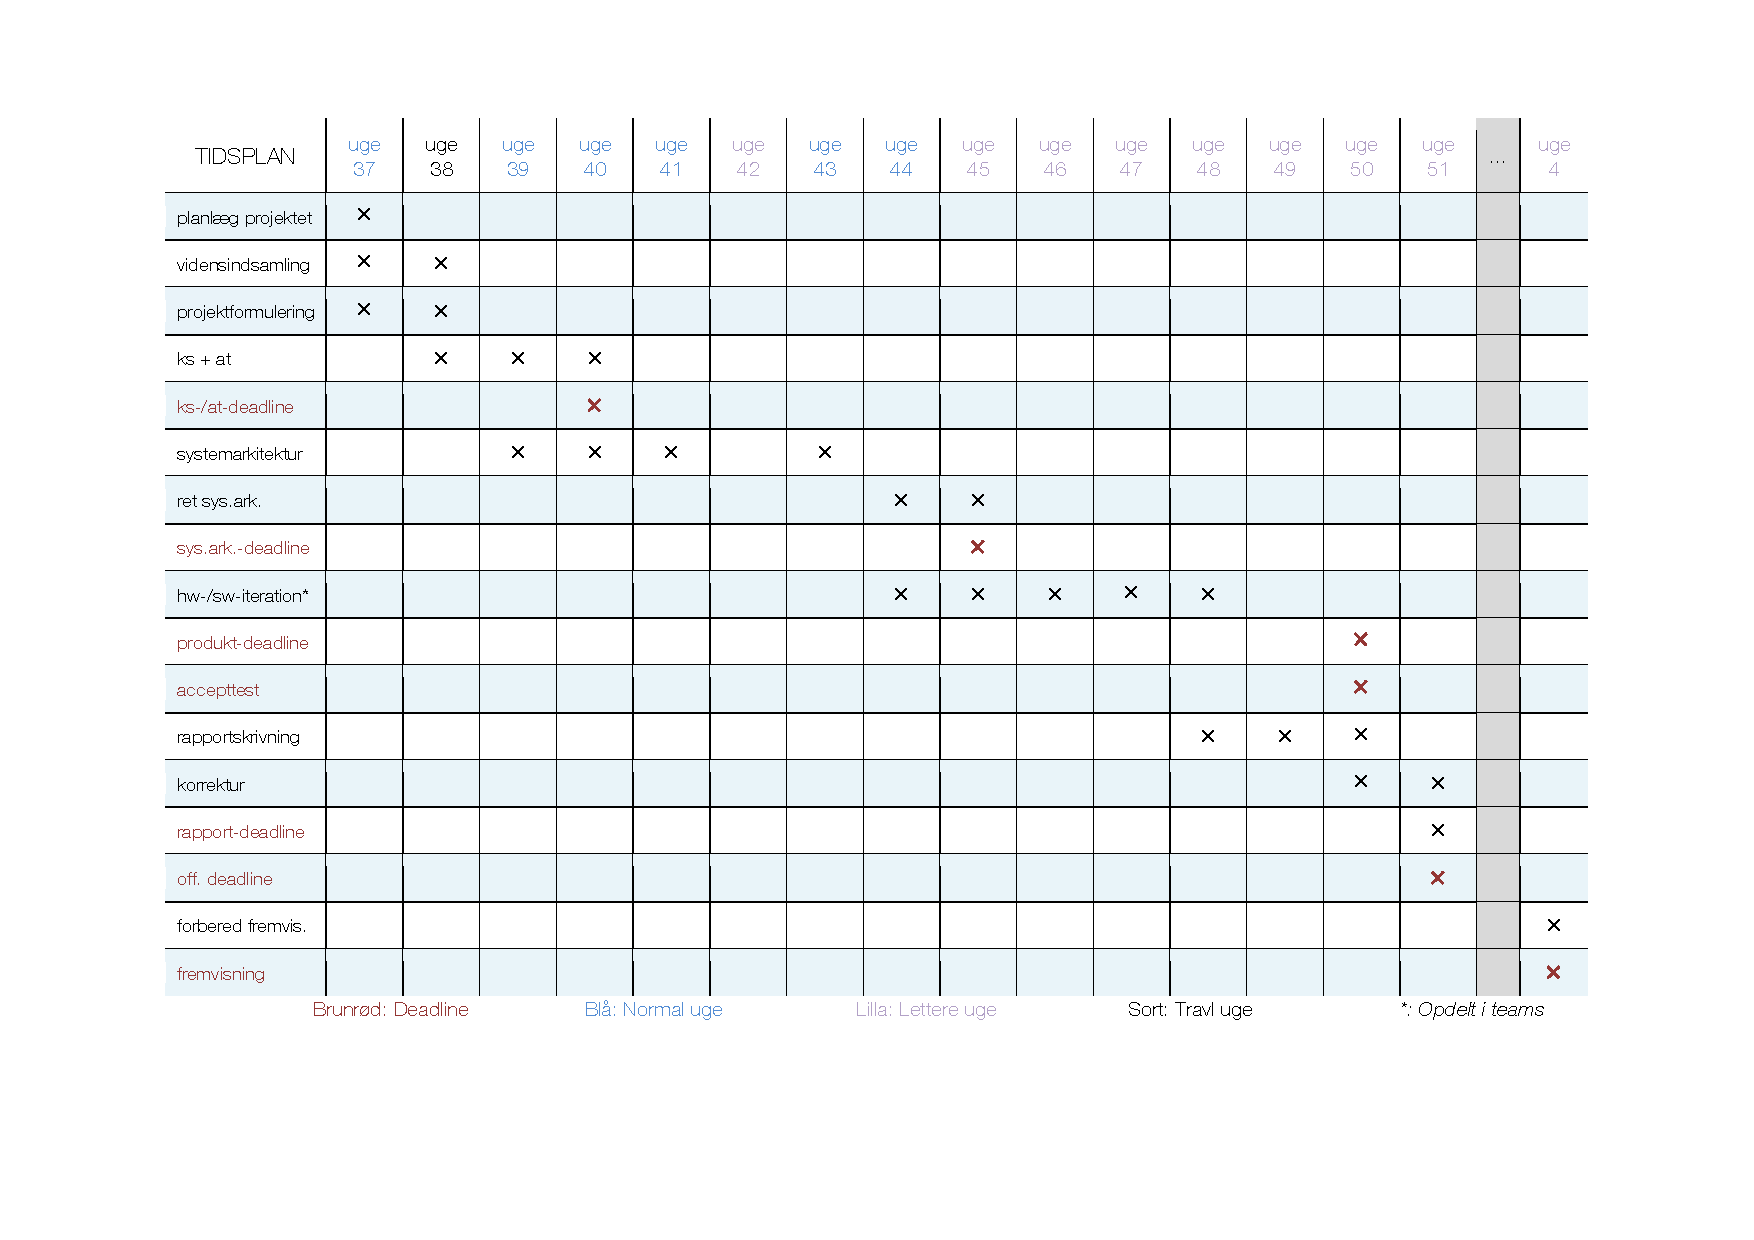
\includegraphics[angle=90]{figurer/Tidsplan}
\end{figure}

\clearpage

\section{Bilag 3: Hardware versioner}\label{bilag3}
\begin{longtabu} to \linewidth{@{}l l l X[j]@{}}
    Version &    Dato &    Ansvarlig &    Beskrivelse\\[-1ex]
    \midrule
    Tekst &    Tekst &    Tekst &    Tekst.\\
    Tekst &    Tekst &    Tekst &    Tekst.\\
    Tekst &    Tekst &    Tekst &    Tekst.\\
    Tekst &    Tekst &    Tekst &    Tekst.\\
\label{version_HW}
\end{longtabu}

\clearpage


\section{Bilag 4: Software versioner}\label{bilag4}
\begin{longtabu} to \linewidth{@{}l l l X[j]@{}}
    Version &    Dato &    Ansvarlig &    Beskrivelse\\[-1ex]
    \midrule
    Tekst &    Tekst &    Tekst &    Tekst.\\
    Tekst &    Tekst &    Tekst &    Tekst.\\
    Tekst &    Tekst &    Tekst &    Tekst.\\
    Tekst &    Tekst &    Tekst &    Tekst.\\
\label{version_SW}
\end{longtabu}

\clearpage

\section{Bilag 5: Logbog}\label{bilag5}
Logbogen findes på vedlagte cd-rom.

\clearpage

\section{Bilag 6: Mødereferater}\label{bilag6}
Mødereferater findes på vedlagte cd-rom.

\clearpage

\section{Bilag 7: Datasheet NI-6009 DAQ}\label{bilag7}
